\documentclass[1p]{elsarticle_modified}
%\bibliographystyle{elsarticle-num}

%\usepackage[colorlinks]{hyperref}
%\usepackage{abbrmath_seonhwa} %\Abb, \Ascr, \Acal ,\Abf, \Afrak
\usepackage{amsfonts}
\usepackage{amssymb}
\usepackage{amsmath}
\usepackage{amsthm}
\usepackage{scalefnt}
\usepackage{amsbsy}
\usepackage{kotex}
\usepackage{caption}
\usepackage{subfig}
\usepackage{color}
\usepackage{graphicx}
\usepackage{xcolor} %% white, black, red, green, blue, cyan, magenta, yellow
\usepackage{float}
\usepackage{setspace}
\usepackage{hyperref}

\usepackage{tikz}
\usetikzlibrary{arrows}

\usepackage{multirow}
\usepackage{array} % fixed length table
\usepackage{hhline}

%%%%%%%%%%%%%%%%%%%%%
\makeatletter
\renewcommand*\env@matrix[1][\arraystretch]{%
	\edef\arraystretch{#1}%
	\hskip -\arraycolsep
	\let\@ifnextchar\new@ifnextchar
	\array{*\c@MaxMatrixCols c}}
\makeatother %https://tex.stackexchange.com/questions/14071/how-can-i-increase-the-line-spacing-in-a-matrix
%%%%%%%%%%%%%%%

\usepackage[normalem]{ulem}

\newcommand{\msout}[1]{\ifmmode\text{\sout{\ensuremath{#1}}}\else\sout{#1}\fi}
%SOURCE: \msout is \stkout macro in https://tex.stackexchange.com/questions/20609/strikeout-in-math-mode

\newcommand{\cancel}[1]{
	\ifmmode
	{\color{red}\msout{#1}}
	\else
	{\color{red}\sout{#1}}
	\fi
}

\newcommand{\add}[1]{
	{\color{blue}\uwave{#1}}
}

\newcommand{\replace}[2]{
	\ifmmode
	{\color{red}\msout{#1}}{\color{blue}\uwave{#2}}
	\else
	{\color{red}\sout{#1}}{\color{blue}\uwave{#2}}
	\fi
}

\newcommand{\Sol}{\mathcal{S}} %segment
\newcommand{\D}{D} %diagram
\newcommand{\A}{\mathcal{A}} %arc


%%%%%%%%%%%%%%%%%%%%%%%%%%%%%5 test

\def\sl{\operatorname{\textup{SL}}(2,\Cbb)}
\def\psl{\operatorname{\textup{PSL}}(2,\Cbb)}
\def\quan{\mkern 1mu \triangleright \mkern 1mu}

\theoremstyle{definition}
\newtheorem{thm}{Theorem}[section]
\newtheorem{prop}[thm]{Proposition}
\newtheorem{lem}[thm]{Lemma}
\newtheorem{ques}[thm]{Question}
\newtheorem{cor}[thm]{Corollary}
\newtheorem{defn}[thm]{Definition}
\newtheorem{exam}[thm]{Example}
\newtheorem{rmk}[thm]{Remark}
\newtheorem{alg}[thm]{Algorithm}

\newcommand{\I}{\sqrt{-1}}
\begin{document}

%\begin{frontmatter}
%
%\title{Boundary parabolic representations of knots up to 8 crossings}
%
%%% Group authors per affiliation:
%\author{Yunhi Cho} 
%\address{Department of Mathematics, University of Seoul, Seoul, Korea}
%\ead{yhcho@uos.ac.kr}
%
%
%\author{Seonhwa Kim} %\fnref{s_kim}}
%\address{Center for Geometry and Physics, Institute for Basic Science, Pohang, 37673, Korea}
%\ead{ryeona17@ibs.re.kr}
%
%\author{Hyuk Kim}
%\address{Department of Mathematical Sciences, Seoul National University, Seoul 08826, Korea}
%\ead{hyukkim@snu.ac.kr}
%
%\author{Seokbeom Yoon}
%\address{Department of Mathematical Sciences, Seoul National University, Seoul, 08826,  Korea}
%\ead{sbyoon15@snu.ac.kr}
%
%\begin{abstract}
%We find all boundary parabolic representation of knots up to 8 crossings.
%
%\end{abstract}
%\begin{keyword}
%    \MSC[2010] 57M25 
%\end{keyword}
%
%\end{frontmatter}

%\linenumbers
%\tableofcontents
%
\newcommand\colored[1]{\textcolor{white}{\rule[-0.35ex]{0.8em}{1.4ex}}\kern-0.8em\color{red} #1}%
%\newcommand\colored[1]{\textcolor{white}{ #1}\kern-2.17ex	\textcolor{white}{ #1}\kern-1.81ex	\textcolor{white}{ #1}\kern-2.15ex\color{red}#1	}

{\Large $\underline{12n_{0495}~(K12n_{0495})}$}

\setlength{\tabcolsep}{10pt}
\renewcommand{\arraystretch}{1.6}
\vspace{1cm}\begin{tabular}{m{100pt}>{\centering\arraybackslash}m{274pt}}
\multirow{5}{120pt}{
	\centering
	\includegraphics[width=112pt]{../../../GIT/diagram.site/Diagrams/png/2584_12n_0495.png}\\
\ \ \ A knot diagram\footnotemark}&
\allowdisplaybreaks
\textbf{Linearized knot diagam} \\
\cline{2-2}
 &
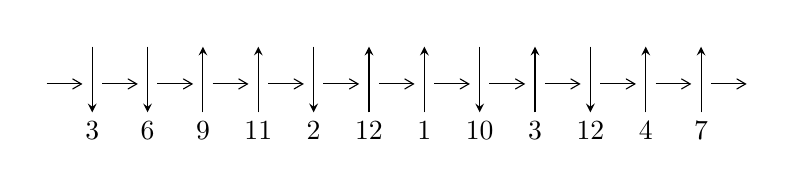
\begin{tikzpicture}[x=20pt, y=17pt]
	% nodes
	\node (C0) at (0, 0) {};
	\node (C1) at (1, 0) {};
	\node (C1U) at (1, +1) {};
	\node (C1D) at (1, -1) {3};

	\node (C2) at (2, 0) {};
	\node (C2U) at (2, +1) {};
	\node (C2D) at (2, -1) {6};

	\node (C3) at (3, 0) {};
	\node (C3U) at (3, +1) {};
	\node (C3D) at (3, -1) {9};

	\node (C4) at (4, 0) {};
	\node (C4U) at (4, +1) {};
	\node (C4D) at (4, -1) {11};

	\node (C5) at (5, 0) {};
	\node (C5U) at (5, +1) {};
	\node (C5D) at (5, -1) {2};

	\node (C6) at (6, 0) {};
	\node (C6U) at (6, +1) {};
	\node (C6D) at (6, -1) {12};

	\node (C7) at (7, 0) {};
	\node (C7U) at (7, +1) {};
	\node (C7D) at (7, -1) {1};

	\node (C8) at (8, 0) {};
	\node (C8U) at (8, +1) {};
	\node (C8D) at (8, -1) {10};

	\node (C9) at (9, 0) {};
	\node (C9U) at (9, +1) {};
	\node (C9D) at (9, -1) {3};

	\node (C10) at (10, 0) {};
	\node (C10U) at (10, +1) {};
	\node (C10D) at (10, -1) {12};

	\node (C11) at (11, 0) {};
	\node (C11U) at (11, +1) {};
	\node (C11D) at (11, -1) {4};

	\node (C12) at (12, 0) {};
	\node (C12U) at (12, +1) {};
	\node (C12D) at (12, -1) {7};
	\node (C13) at (13, 0) {};

	% arrows
	\draw[->,>={angle 60}]
	(C0) edge (C1) (C1) edge (C2) (C2) edge (C3) (C3) edge (C4) (C4) edge (C5) (C5) edge (C6) (C6) edge (C7) (C7) edge (C8) (C8) edge (C9) (C9) edge (C10) (C10) edge (C11) (C11) edge (C12) (C12) edge (C13) ;	\draw[->,>=stealth]
	(C1U) edge (C1D) (C2U) edge (C2D) (C3D) edge (C3U) (C4D) edge (C4U) (C5U) edge (C5D) (C6D) edge (C6U) (C7D) edge (C7U) (C8U) edge (C8D) (C9D) edge (C9U) (C10U) edge (C10D) (C11D) edge (C11U) (C12D) edge (C12U) ;
	\end{tikzpicture} \\
\hhline{~~} \\& 
\textbf{Solving Sequence} \\ \cline{2-2} 
 &
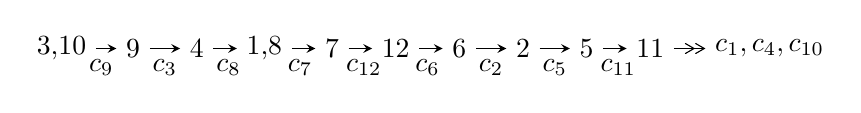
\begin{tikzpicture}[x=23pt, y=7pt]
	% node
	\node (A0) at (-1/8, 0) {3,10};
	\node (A1) at (1, 0) {9};
	\node (A2) at (2, 0) {4};
	\node (A3) at (49/16, 0) {1,8};
	\node (A4) at (33/8, 0) {7};
	\node (A5) at (41/8, 0) {12};
	\node (A6) at (49/8, 0) {6};
	\node (A7) at (57/8, 0) {2};
	\node (A8) at (65/8, 0) {5};
	\node (A9) at (73/8, 0) {11};
	\node (C1) at (1/2, -1) {$c_{9}$};
	\node (C2) at (3/2, -1) {$c_{3}$};
	\node (C3) at (5/2, -1) {$c_{8}$};
	\node (C4) at (29/8, -1) {$c_{7}$};
	\node (C5) at (37/8, -1) {$c_{12}$};
	\node (C6) at (45/8, -1) {$c_{6}$};
	\node (C7) at (53/8, -1) {$c_{2}$};
	\node (C8) at (61/8, -1) {$c_{5}$};
	\node (C9) at (69/8, -1) {$c_{11}$};
	\node (A10) at (11, 0) {$c_{1},c_{4},c_{10}$};

	% edge
	\draw[->,>=stealth]	
	(A0) edge (A1) (A1) edge (A2) (A2) edge (A3) (A3) edge (A4) (A4) edge (A5) (A5) edge (A6) (A6) edge (A7) (A7) edge (A8) (A8) edge (A9) ;
	\draw[->>,>={angle 60}]	
	(A9) edge (A10);
\end{tikzpicture} \\ 

\end{tabular} \\

\footnotetext{
The image of knot diagram is generated by the software ``\textbf{Draw programme}" developed by Andrew Bartholomew(\url{http://www.layer8.co.uk/maths/draw/index.htm\#Running-draw}), where we modified some parts for our purpose(\url{https://github.com/CATsTAILs/LinksPainter}).
}\phantom \\ \newline 
\centering \textbf{Ideals for irreducible components\footnotemark of $X_{\text{par}}$} 
 
\begin{align*}
I^u_{1}&=\langle 
5 u^{14}-18 u^{13}+\cdots+32 b-6,\;10 u^{14}-33 u^{13}+\cdots+16 a-24,\\
\phantom{I^u_{1}}&\phantom{= \langle  }u^{15}-3 u^{14}+7 u^{13}-11 u^{12}+26 u^{11}-40 u^{10}+58 u^9-56 u^8+77 u^7-59 u^6+55 u^5-15 u^4+16 u^3+6 u^2+2\rangle \\
I^u_{2}&=\langle 
u^3+u^2+2 b,\;u^3+2 a+u,\;u^4+u^2+2\rangle \\
I^u_{3}&=\langle 
-71485 u^{13}-71179 u^{12}+\cdots+855248 b-1081596,\\
\phantom{I^u_{3}}&\phantom{= \langle  }-61525 u^{13}+23653 u^{12}+\cdots+1710496 a+2423156,\\
\phantom{I^u_{3}}&\phantom{= \langle  }u^{14}+u^{13}+u^{12}+7 u^{11}+12 u^{10}+12 u^9+36 u^8+46 u^7+51 u^6+89 u^5+73 u^4+57 u^3+58 u^2+12 u+8\rangle \\
I^u_{4}&=\langle 
- a^3 u- a^3+2 a^2+3 a u+2 b+a- u-3,\;a^4+a^3 u-3 a^2-2 a u+1,\;u^2+1\rangle \\
I^u_{5}&=\langle 
- a^2+4 b-3 a,\;a^3+2 a^2+a+4,\;u+1\rangle \\
I^u_{6}&=\langle 
u^3- u^2+2 b- u+1,\;u^3+a,\;u^4+1\rangle \\
\\
I^v_{1}&=\langle 
a,\;b+1,\;v-1\rangle \\
\end{align*}
\raggedright * 7 irreducible components of $\dim_{\mathbb{C}}=0$, with total 49 representations.\\
\footnotetext{All coefficients of polynomials are rational numbers. But the coefficients are sometimes approximated in decimal forms when there is not enough margin.}
\newpage
\renewcommand{\arraystretch}{1}
\centering \section*{I. $I^u_{1}= \langle 5 u^{14}-18 u^{13}+\cdots+32 b-6,\;10 u^{14}-33 u^{13}+\cdots+16 a-24,\;u^{15}-3 u^{14}+\cdots+6 u^2+2 \rangle$}
\flushleft \textbf{(i) Arc colorings}\\
\begin{tabular}{m{7pt} m{180pt} m{7pt} m{180pt} }
\flushright $a_{3}=$&$\begin{pmatrix}0\\u\end{pmatrix}$ \\
\flushright $a_{10}=$&$\begin{pmatrix}1\\0\end{pmatrix}$ \\
\flushright $a_{9}=$&$\begin{pmatrix}1\\u^2\end{pmatrix}$ \\
\flushright $a_{4}=$&$\begin{pmatrix}u\\u^3+u\end{pmatrix}$ \\
\flushright $a_{1}=$&$\begin{pmatrix}-\frac{5}{8} u^{14}+\frac{33}{16} u^{13}+\cdots-\frac{23}{8} u+\frac{3}{2}\\-0.156250 u^{14}+0.562500 u^{13}+\cdots-0.312500 u+0.187500\end{pmatrix}$ \\
\flushright $a_{8}=$&$\begin{pmatrix}u^2+1\\u^2\end{pmatrix}$ \\
\flushright $a_{7}=$&$\begin{pmatrix}\frac{1}{16} u^{14}-\frac{1}{2} u^{13}+\cdots-\frac{7}{8} u+\frac{1}{8}\\0.156250 u^{14}-0.562500 u^{13}+\cdots+0.312500 u-0.187500\end{pmatrix}$ \\
\flushright $a_{12}=$&$\begin{pmatrix}-\frac{1}{8} u^{13}+\frac{3}{8} u^{12}+\cdots-\frac{5}{2} u^2+\frac{3}{4}\\- u^2\end{pmatrix}$ \\
\flushright $a_{6}=$&$\begin{pmatrix}-\frac{9}{16} u^{14}+\frac{7}{4} u^{13}+\cdots-4 u+\frac{3}{2}\\\frac{1}{32} u^{14}-\frac{1}{8} u^{13}+\cdots-\frac{5}{16} u+\frac{1}{16}\end{pmatrix}$ \\
\flushright $a_{2}=$&$\begin{pmatrix}-\frac{5}{8} u^{14}+\frac{33}{16} u^{13}+\cdots-\frac{23}{8} u+\frac{3}{2}\\\frac{1}{32} u^{14}-\frac{1}{8} u^{13}+\cdots+\frac{15}{16} u-\frac{3}{16}\end{pmatrix}$ \\
\flushright $a_{5}=$&$\begin{pmatrix}\frac{1}{8} u^{14}-\frac{3}{8} u^{13}+\cdots+\frac{3}{2} u^3-\frac{7}{4} u\\- u^5- u^3- u\end{pmatrix}$ \\
\flushright $a_{11}=$&$\begin{pmatrix}-\frac{1}{8} u^{13}+\frac{3}{8} u^{12}+\cdots-\frac{3}{2} u^2+\frac{3}{4}\\u^4\end{pmatrix}$\\&\end{tabular}
\flushleft \textbf{(ii) Obstruction class $= -1$}\\~\\
\flushleft \textbf{(iii) Cusp Shapes $= \frac{17}{8} u^{14}-\frac{27}{4} u^{13}+\frac{125}{8} u^{12}-\frac{99}{4} u^{11}+\frac{113}{2} u^{10}-\frac{181}{2} u^9+\frac{515}{4} u^8-\frac{501}{4} u^7+\frac{1299}{8} u^6-\frac{273}{2} u^5+\frac{927}{8} u^4-34 u^3+20 u^2+\frac{11}{4} u-\frac{1}{4}$}\\~\\
\newpage\renewcommand{\arraystretch}{1}
\flushleft \textbf{(iv) u-Polynomials at the component}\newline \\
\begin{tabular}{m{50pt}|m{274pt}}
Crossings & \hspace{64pt}u-Polynomials at each crossing \\
\hline $$\begin{aligned}c_{1}\end{aligned}$$&$\begin{aligned}
&u^{15}+18 u^{13}+\cdots+1061 u+121
\end{aligned}$\\
\hline $$\begin{aligned}c_{2},c_{5}\end{aligned}$$&$\begin{aligned}
&u^{15}+6 u^{14}+\cdots+7 u-11
\end{aligned}$\\
\hline $$\begin{aligned}c_{3},c_{4},c_{9}\\c_{11}\end{aligned}$$&$\begin{aligned}
&u^{15}+3 u^{14}+\cdots-6 u^2-2
\end{aligned}$\\
\hline $$\begin{aligned}c_{6},c_{7},c_{12}\end{aligned}$$&$\begin{aligned}
&u^{15}-6 u^{14}+\cdots-5 u-11
\end{aligned}$\\
\hline $$\begin{aligned}c_{8},c_{10}\end{aligned}$$&$\begin{aligned}
&u^{15}+5 u^{14}+\cdots-24 u-4
\end{aligned}$\\
\hline
\end{tabular}\\~\\
\newpage\renewcommand{\arraystretch}{1}
\flushleft \textbf{(v) Riley Polynomials at the component}\newline \\
\begin{tabular}{m{50pt}|m{274pt}}
Crossings & \hspace{64pt}Riley Polynomials at each crossing \\
\hline $$\begin{aligned}c_{1}\end{aligned}$$&$\begin{aligned}
&y^{15}+36 y^{14}+\cdots+486357 y-14641
\end{aligned}$\\
\hline $$\begin{aligned}c_{2},c_{5}\end{aligned}$$&$\begin{aligned}
&y^{15}+18 y^{13}+\cdots+1061 y-121
\end{aligned}$\\
\hline $$\begin{aligned}c_{3},c_{4},c_{9}\\c_{11}\end{aligned}$$&$\begin{aligned}
&y^{15}+5 y^{14}+\cdots-24 y-4
\end{aligned}$\\
\hline $$\begin{aligned}c_{6},c_{7},c_{12}\end{aligned}$$&$\begin{aligned}
&y^{15}-24 y^{14}+\cdots-459 y-121
\end{aligned}$\\
\hline $$\begin{aligned}c_{8},c_{10}\end{aligned}$$&$\begin{aligned}
&y^{15}+45 y^{14}+\cdots+768 y-16
\end{aligned}$\\
\hline
\end{tabular}\\~\\
\newpage\flushleft \textbf{(vi) Complex Volumes and Cusp Shapes}
$$\begin{array}{c|c|c}  
\text{Solutions to }I^u_{1}& \I (\text{vol} + \sqrt{-1}CS) & \text{Cusp shape}\\
 \hline 
\begin{aligned}
u &= \phantom{-}0.697385 + 0.828178 I \\
a &= \phantom{-}0.320085 - 1.205310 I \\
b &= \phantom{-}0.596828 - 0.784304 I\end{aligned}
 & -1.30143 + 4.86126 I & -1.54571 - 6.09014 I \\ \hline\begin{aligned}
u &= \phantom{-}0.697385 - 0.828178 I \\
a &= \phantom{-}0.320085 + 1.205310 I \\
b &= \phantom{-}0.596828 + 0.784304 I\end{aligned}
 & -1.30143 - 4.86126 I & -1.54571 + 6.09014 I \\ \hline\begin{aligned}
u &= -0.568338 + 1.053040 I \\
a &= \phantom{-}0.458588 - 0.214607 I \\
b &= \phantom{-}0.355345 + 0.509744 I\end{aligned}
 & \phantom{-}2.62859 - 6.17338 I & \phantom{-}5.25348 + 7.15560 I \\ \hline\begin{aligned}
u &= -0.568338 - 1.053040 I \\
a &= \phantom{-}0.458588 + 0.214607 I \\
b &= \phantom{-}0.355345 - 0.509744 I\end{aligned}
 & \phantom{-}2.62859 + 6.17338 I & \phantom{-}5.25348 - 7.15560 I \\ \hline\begin{aligned}
u &= -0.059276 + 0.727915 I \\
a &= -1.94701 - 0.12490 I \\
b &= -1.037900 + 0.063892 I\end{aligned}
 & \phantom{-}4.57881 + 2.95035 I & \phantom{-}8.93827 - 0.98271 I \\ \hline\begin{aligned}
u &= -0.059276 - 0.727915 I \\
a &= -1.94701 + 0.12490 I \\
b &= -1.037900 - 0.063892 I\end{aligned}
 & \phantom{-}4.57881 - 2.95035 I & \phantom{-}8.93827 + 0.98271 I \\ \hline\begin{aligned}
u &= \phantom{-}0.142281 + 0.483742 I \\
a &= \phantom{-}1.39721 - 0.99957 I \\
b &= \phantom{-}0.178761 - 0.047955 I\end{aligned}
 & -1.49033 - 1.08782 I & -1.21432 + 1.45793 I \\ \hline\begin{aligned}
u &= \phantom{-}0.142281 - 0.483742 I \\
a &= \phantom{-}1.39721 + 0.99957 I \\
b &= \phantom{-}0.178761 + 0.047955 I\end{aligned}
 & -1.49033 + 1.08782 I & -1.21432 - 1.45793 I \\ \hline\begin{aligned}
u &= \phantom{-}1.18615 + 1.00645 I \\
a &= -1.46570 - 0.18514 I \\
b &= -0.570924 - 0.788977 I\end{aligned}
 & \phantom{-}6.77956 + 6.79736 I & \phantom{-}4.43994 - 4.51085 I \\ \hline\begin{aligned}
u &= \phantom{-}1.18615 - 1.00645 I \\
a &= -1.46570 + 0.18514 I \\
b &= -0.570924 + 0.788977 I\end{aligned}
 & \phantom{-}6.77956 - 6.79736 I & \phantom{-}4.43994 + 4.51085 I\\
 \hline 
 \end{array}$$\newpage$$\begin{array}{c|c|c}  
\text{Solutions to }I^u_{1}& \I (\text{vol} + \sqrt{-1}CS) & \text{Cusp shape}\\
 \hline 
\begin{aligned}
u &= -0.423770\phantom{ +0.000000I} \\
a &= -0.380234\phantom{ +0.000000I} \\
b &= -0.682622\phantom{ +0.000000I}\end{aligned}
 & \phantom{-}0.948533\phantom{ +0.000000I} & \phantom{-}11.8010\phantom{ +0.000000I} \\ \hline\begin{aligned}
u &= -0.90624 + 1.36309 I \\
a &= \phantom{-}1.16372 - 1.52636 I \\
b &= \phantom{-}0.36666 - 2.75118 I\end{aligned}
 & \phantom{-}16.2386 - 13.6992 I & \phantom{-}2.92416 + 5.89399 I \\ \hline\begin{aligned}
u &= -0.90624 - 1.36309 I \\
a &= \phantom{-}1.16372 + 1.52636 I \\
b &= \phantom{-}0.36666 + 2.75118 I\end{aligned}
 & \phantom{-}16.2386 + 13.6992 I & \phantom{-}2.92416 - 5.89399 I \\ \hline\begin{aligned}
u &= \phantom{-}1.21992 + 1.30757 I \\
a &= \phantom{-}0.76322 + 1.95846 I \\
b &= -0.04746 + 2.68598 I\end{aligned}
 & \phantom{-}18.1501 + 4.1175 I & \phantom{-}4.30382 - 1.81660 I \\ \hline\begin{aligned}
u &= \phantom{-}1.21992 - 1.30757 I \\
a &= \phantom{-}0.76322 - 1.95846 I \\
b &= -0.04746 - 2.68598 I\end{aligned}
 & \phantom{-}18.1501 - 4.1175 I & \phantom{-}4.30382 + 1.81660 I\\
 \hline 
 \end{array}$$\newpage\newpage\renewcommand{\arraystretch}{1}
\centering \section*{II. $I^u_{2}= \langle u^3+u^2+2 b,\;u^3+2 a+u,\;u^4+u^2+2 \rangle$}
\flushleft \textbf{(i) Arc colorings}\\
\begin{tabular}{m{7pt} m{180pt} m{7pt} m{180pt} }
\flushright $a_{3}=$&$\begin{pmatrix}0\\u\end{pmatrix}$ \\
\flushright $a_{10}=$&$\begin{pmatrix}1\\0\end{pmatrix}$ \\
\flushright $a_{9}=$&$\begin{pmatrix}1\\u^2\end{pmatrix}$ \\
\flushright $a_{4}=$&$\begin{pmatrix}u\\u^3+u\end{pmatrix}$ \\
\flushright $a_{1}=$&$\begin{pmatrix}-\frac{1}{2} u^3-\frac{1}{2} u\\-\frac{1}{2} u^3-\frac{1}{2} u^2\end{pmatrix}$ \\
\flushright $a_{8}=$&$\begin{pmatrix}u^2+1\\u^2\end{pmatrix}$ \\
\flushright $a_{7}=$&$\begin{pmatrix}-\frac{1}{2} u^3+u^2-\frac{1}{2} u+1\\-\frac{1}{2} u^3+\frac{1}{2} u^2\end{pmatrix}$ \\
\flushright $a_{12}=$&$\begin{pmatrix}- u^2-1\\- u^2\end{pmatrix}$ \\
\flushright $a_{6}=$&$\begin{pmatrix}-\frac{1}{2} u^3-\frac{1}{2} u\\-\frac{1}{2} u^3-\frac{1}{2} u^2\end{pmatrix}$ \\
\flushright $a_{2}=$&$\begin{pmatrix}-\frac{1}{2} u^3-\frac{1}{2} u\\-\frac{1}{2} u^3-\frac{1}{2} u^2+u\end{pmatrix}$ \\
\flushright $a_{5}=$&$\begin{pmatrix}0\\- u\end{pmatrix}$ \\
\flushright $a_{11}=$&$\begin{pmatrix}-1\\- u^2-2\end{pmatrix}$\\&\end{tabular}
\flushleft \textbf{(ii) Obstruction class $= 1$}\\~\\
\flushleft \textbf{(iii) Cusp Shapes $= -4 u^2$}\\~\\
\newpage\renewcommand{\arraystretch}{1}
\flushleft \textbf{(iv) u-Polynomials at the component}\newline \\
\begin{tabular}{m{50pt}|m{274pt}}
Crossings & \hspace{64pt}u-Polynomials at each crossing \\
\hline $$\begin{aligned}c_{1},c_{5},c_{6}\\c_{7}\end{aligned}$$&$\begin{aligned}
&(u-1)^4
\end{aligned}$\\
\hline $$\begin{aligned}c_{2},c_{12}\end{aligned}$$&$\begin{aligned}
&(u+1)^4
\end{aligned}$\\
\hline $$\begin{aligned}c_{3},c_{4},c_{9}\\c_{11}\end{aligned}$$&$\begin{aligned}
&u^4+u^2+2
\end{aligned}$\\
\hline $$\begin{aligned}c_{8},c_{10}\end{aligned}$$&$\begin{aligned}
&(u^2- u+2)^2
\end{aligned}$\\
\hline
\end{tabular}\\~\\
\newpage\renewcommand{\arraystretch}{1}
\flushleft \textbf{(v) Riley Polynomials at the component}\newline \\
\begin{tabular}{m{50pt}|m{274pt}}
Crossings & \hspace{64pt}Riley Polynomials at each crossing \\
\hline $$\begin{aligned}c_{1},c_{2},c_{5}\\c_{6},c_{7},c_{12}\end{aligned}$$&$\begin{aligned}
&(y-1)^4
\end{aligned}$\\
\hline $$\begin{aligned}c_{3},c_{4},c_{9}\\c_{11}\end{aligned}$$&$\begin{aligned}
&(y^2+y+2)^2
\end{aligned}$\\
\hline $$\begin{aligned}c_{8},c_{10}\end{aligned}$$&$\begin{aligned}
&(y^2+3 y+4)^2
\end{aligned}$\\
\hline
\end{tabular}\\~\\
\newpage\flushleft \textbf{(vi) Complex Volumes and Cusp Shapes}
$$\begin{array}{c|c|c}  
\text{Solutions to }I^u_{2}& \I (\text{vol} + \sqrt{-1}CS) & \text{Cusp shape}\\
 \hline 
\begin{aligned}
u &= \phantom{-}0.676097 + 0.978318 I \\
a &= \phantom{-}0.478073 - 0.691776 I \\
b &= \phantom{-}1.066120 - 0.864054 I\end{aligned}
 & \phantom{-}0.82247 + 5.33349 I & \phantom{-}2.00000 - 5.29150 I \\ \hline\begin{aligned}
u &= \phantom{-}0.676097 - 0.978318 I \\
a &= \phantom{-}0.478073 + 0.691776 I \\
b &= \phantom{-}1.066120 + 0.864054 I\end{aligned}
 & \phantom{-}0.82247 - 5.33349 I & \phantom{-}2.00000 + 5.29150 I \\ \hline\begin{aligned}
u &= -0.676097 + 0.978318 I \\
a &= -0.478073 - 0.691776 I \\
b &= -0.566121 + 0.458821 I\end{aligned}
 & \phantom{-}0.82247 - 5.33349 I & \phantom{-}2.00000 + 5.29150 I \\ \hline\begin{aligned}
u &= -0.676097 - 0.978318 I \\
a &= -0.478073 + 0.691776 I \\
b &= -0.566121 - 0.458821 I\end{aligned}
 & \phantom{-}0.82247 + 5.33349 I & \phantom{-}2.00000 - 5.29150 I\\
 \hline 
 \end{array}$$\newpage\newpage\renewcommand{\arraystretch}{1}
\centering \section*{III. $I^u_{3}= \langle -7.15\times10^{4} u^{13}-7.12\times10^{4} u^{12}+\cdots+8.55\times10^{5} b-1.08\times10^{6},\;-6.15\times10^{4} u^{13}+2.37\times10^{4} u^{12}+\cdots+1.71\times10^{6} a+2.42\times10^{6},\;u^{14}+u^{13}+\cdots+12 u+8 \rangle$}
\flushleft \textbf{(i) Arc colorings}\\
\begin{tabular}{m{7pt} m{180pt} m{7pt} m{180pt} }
\flushright $a_{3}=$&$\begin{pmatrix}0\\u\end{pmatrix}$ \\
\flushright $a_{10}=$&$\begin{pmatrix}1\\0\end{pmatrix}$ \\
\flushright $a_{9}=$&$\begin{pmatrix}1\\u^2\end{pmatrix}$ \\
\flushright $a_{4}=$&$\begin{pmatrix}u\\u^3+u\end{pmatrix}$ \\
\flushright $a_{1}=$&$\begin{pmatrix}0.0359691 u^{13}-0.0138282 u^{12}+\cdots-0.612814 u-1.41664\\0.0835839 u^{13}+0.0832262 u^{12}+\cdots+2.37555 u+1.26466\end{pmatrix}$ \\
\flushright $a_{8}=$&$\begin{pmatrix}u^2+1\\u^2\end{pmatrix}$ \\
\flushright $a_{7}=$&$\begin{pmatrix}-0.0716091 u^{13}-0.0864036 u^{12}+\cdots-2.69890 u-0.496032\\0.0256803 u^{13}+0.0829128 u^{12}+\cdots+3.52899 u+1.16024\end{pmatrix}$ \\
\flushright $a_{12}=$&$\begin{pmatrix}0.0423257 u^{13}+0.0196119 u^{12}+\cdots+0.694498 u-1.67568\\-0.00489683 u^{13}-0.000238527 u^{12}+\cdots-0.0660393 u+1.18171\end{pmatrix}$ \\
\flushright $a_{6}=$&$\begin{pmatrix}-0.0923358 u^{13}-0.177850 u^{12}+\cdots-4.80626 u-2.20422\\0.0564421 u^{13}+0.128466 u^{12}+\cdots+5.94481 u+2.59514\end{pmatrix}$ \\
\flushright $a_{2}=$&$\begin{pmatrix}0.0359691 u^{13}-0.0138282 u^{12}+\cdots-0.612814 u-1.41664\\0.105884 u^{13}+0.0653296 u^{12}+\cdots+2.68537 u+1.66304\end{pmatrix}$ \\
\flushright $a_{5}=$&$\begin{pmatrix}-0.120342 u^{13}-0.180647 u^{12}+\cdots-6.00953 u-1.46083\\0.0761440 u^{13}+0.0459726 u^{12}+\cdots+5.11046 u+0.860223\end{pmatrix}$ \\
\flushright $a_{11}=$&$\begin{pmatrix}0.0374289 u^{13}+0.0193733 u^{12}+\cdots+0.628459 u-1.49397\\-0.0700990 u^{13}-0.0120106 u^{12}+\cdots-0.148804 u+1.32616\end{pmatrix}$\\&\end{tabular}
\flushleft \textbf{(ii) Obstruction class $= -1$}\\~\\
\flushleft \textbf{(iii) Cusp Shapes $= -\frac{133137}{213812} u^{13}-\frac{52127}{213812} u^{12}+\cdots-\frac{496203}{53453} u+\frac{335445}{53453}$}\\~\\
\newpage\renewcommand{\arraystretch}{1}
\flushleft \textbf{(iv) u-Polynomials at the component}\newline \\
\begin{tabular}{m{50pt}|m{274pt}}
Crossings & \hspace{64pt}u-Polynomials at each crossing \\
\hline $$\begin{aligned}c_{1}\end{aligned}$$&$\begin{aligned}
&(u^7-2 u^6+15 u^5-35 u^4+11 u^3+20 u^2+13 u+9)^2
\end{aligned}$\\
\hline $$\begin{aligned}c_{2},c_{5}\end{aligned}$$&$\begin{aligned}
&(u^7-2 u^6+3 u^5- u^4+5 u^3+2 u^2- u-3)^2
\end{aligned}$\\
\hline $$\begin{aligned}c_{3},c_{4},c_{9}\\c_{11}\end{aligned}$$&$\begin{aligned}
&u^{14}- u^{13}+\cdots-12 u+8
\end{aligned}$\\
\hline $$\begin{aligned}c_{6},c_{7},c_{12}\end{aligned}$$&$\begin{aligned}
&(u^7+2 u^6-5 u^5-9 u^4+9 u^3+14 u^2+3 u-3)^2
\end{aligned}$\\
\hline $$\begin{aligned}c_{8},c_{10}\end{aligned}$$&$\begin{aligned}
&u^{14}+u^{13}+\cdots+784 u+64
\end{aligned}$\\
\hline
\end{tabular}\\~\\
\newpage\renewcommand{\arraystretch}{1}
\flushleft \textbf{(v) Riley Polynomials at the component}\newline \\
\begin{tabular}{m{50pt}|m{274pt}}
Crossings & \hspace{64pt}Riley Polynomials at each crossing \\
\hline $$\begin{aligned}c_{1}\end{aligned}$$&$\begin{aligned}
&(y^7+26 y^6+107 y^5-789 y^4+1947 y^3+516 y^2-191 y-81)^2
\end{aligned}$\\
\hline $$\begin{aligned}c_{2},c_{5}\end{aligned}$$&$\begin{aligned}
&(y^7+2 y^6+15 y^5+35 y^4+11 y^3-20 y^2+13 y-9)^2
\end{aligned}$\\
\hline $$\begin{aligned}c_{3},c_{4},c_{9}\\c_{11}\end{aligned}$$&$\begin{aligned}
&y^{14}+y^{13}+\cdots+784 y+64
\end{aligned}$\\
\hline $$\begin{aligned}c_{6},c_{7},c_{12}\end{aligned}$$&$\begin{aligned}
&(y^7-14 y^6+79 y^5-221 y^4+315 y^3-196 y^2+93 y-9)^2
\end{aligned}$\\
\hline $$\begin{aligned}c_{8},c_{10}\end{aligned}$$&$\begin{aligned}
&y^{14}+21 y^{13}+\cdots-209664 y+4096
\end{aligned}$\\
\hline
\end{tabular}\\~\\
\newpage\flushleft \textbf{(vi) Complex Volumes and Cusp Shapes}
$$\begin{array}{c|c|c}  
\text{Solutions to }I^u_{3}& \I (\text{vol} + \sqrt{-1}CS) & \text{Cusp shape}\\
 \hline 
\begin{aligned}
u &= \phantom{-}0.189350 + 1.052410 I \\
a &= \phantom{-}0.100138 - 0.556568 I \\
b &= \phantom{-}1.64987 + 0.29513 I\end{aligned}
 & -4.30745\phantom{ +0.000000I} & -7.31983 + 0. I\phantom{ +0.000000I} \\ \hline\begin{aligned}
u &= \phantom{-}0.189350 - 1.052410 I \\
a &= \phantom{-}0.100138 + 0.556568 I \\
b &= \phantom{-}1.64987 - 0.29513 I\end{aligned}
 & -4.30745\phantom{ +0.000000I} & -7.31983 + 0. I\phantom{ +0.000000I} \\ \hline\begin{aligned}
u &= \phantom{-}0.009734 + 1.144270 I \\
a &= \phantom{-}0.482951 - 0.115663 I \\
b &= -0.207824 + 0.900142 I\end{aligned}
 & -2.06755 - 1.45738 I & \phantom{-}4.50826 + 4.10370 I \\ \hline\begin{aligned}
u &= \phantom{-}0.009734 - 1.144270 I \\
a &= \phantom{-}0.482951 + 0.115663 I \\
b &= -0.207824 - 0.900142 I\end{aligned}
 & -2.06755 + 1.45738 I & \phantom{-}4.50826 - 4.10370 I \\ \hline\begin{aligned}
u &= -1.185310 + 0.249865 I \\
a &= \phantom{-}1.21841 + 0.75477 I \\
b &= \phantom{-}0.108273 + 0.365843 I\end{aligned}
 & \phantom{-}5.47090 + 1.03782 I & \phantom{-}5.54723 - 0.70964 I \\ \hline\begin{aligned}
u &= -1.185310 - 0.249865 I \\
a &= \phantom{-}1.21841 - 0.75477 I \\
b &= \phantom{-}0.108273 - 0.365843 I\end{aligned}
 & \phantom{-}5.47090 - 1.03782 I & \phantom{-}5.54723 + 0.70964 I \\ \hline\begin{aligned}
u &= \phantom{-}0.74851 + 1.30026 I \\
a &= -0.883878 + 0.746918 I \\
b &= -0.98455 + 1.12797 I\end{aligned}
 & \phantom{-}5.47090 + 1.03782 I & \phantom{-}5.54723 - 0.70964 I \\ \hline\begin{aligned}
u &= \phantom{-}0.74851 - 1.30026 I \\
a &= -0.883878 - 0.746918 I \\
b &= -0.98455 - 1.12797 I\end{aligned}
 & \phantom{-}5.47090 - 1.03782 I & \phantom{-}5.54723 + 0.70964 I \\ \hline\begin{aligned}
u &= -0.062057 + 0.426068 I \\
a &= -1.313380 - 0.130369 I \\
b &= \phantom{-}1.048580 + 0.721441 I\end{aligned}
 & -2.06755 + 1.45738 I & \phantom{-}4.50826 - 4.10370 I \\ \hline\begin{aligned}
u &= -0.062057 - 0.426068 I \\
a &= -1.313380 + 0.130369 I \\
b &= \phantom{-}1.048580 - 0.721441 I\end{aligned}
 & -2.06755 - 1.45738 I & \phantom{-}4.50826 + 4.10370 I\\
 \hline 
 \end{array}$$\newpage$$\begin{array}{c|c|c}  
\text{Solutions to }I^u_{3}& \I (\text{vol} + \sqrt{-1}CS) & \text{Cusp shape}\\
 \hline 
\begin{aligned}
u &= -1.48947 + 0.77264 I \\
a &= -1.17405 + 2.01302 I \\
b &= -0.15440 + 2.28010 I\end{aligned}
 & \phantom{-}18.4896 + 5.2126 I & \phantom{-}4.60442 - 1.93466 I \\ \hline\begin{aligned}
u &= -1.48947 - 0.77264 I \\
a &= -1.17405 - 2.01302 I \\
b &= -0.15440 - 2.28010 I\end{aligned}
 & \phantom{-}18.4896 - 5.2126 I & \phantom{-}4.60442 + 1.93466 I \\ \hline\begin{aligned}
u &= \phantom{-}1.28924 + 1.19882 I \\
a &= -1.43019 - 1.69938 I \\
b &= -0.45995 - 2.46137 I\end{aligned}
 & \phantom{-}18.4896 + 5.2126 I & \phantom{-}4.60442 - 1.93466 I \\ \hline\begin{aligned}
u &= \phantom{-}1.28924 - 1.19882 I \\
a &= -1.43019 + 1.69938 I \\
b &= -0.45995 + 2.46137 I\end{aligned}
 & \phantom{-}18.4896 - 5.2126 I & \phantom{-}4.60442 + 1.93466 I\\
 \hline 
 \end{array}$$\newpage\newpage\renewcommand{\arraystretch}{1}
\centering \section*{IV. $I^u_{4}= \langle - a^3 u- a^3+2 a^2+3 a u+2 b+a- u-3,\;a^4+a^3 u-3 a^2-2 a u+1,\;u^2+1 \rangle$}
\flushleft \textbf{(i) Arc colorings}\\
\begin{tabular}{m{7pt} m{180pt} m{7pt} m{180pt} }
\flushright $a_{3}=$&$\begin{pmatrix}0\\u\end{pmatrix}$ \\
\flushright $a_{10}=$&$\begin{pmatrix}1\\0\end{pmatrix}$ \\
\flushright $a_{9}=$&$\begin{pmatrix}1\\-1\end{pmatrix}$ \\
\flushright $a_{4}=$&$\begin{pmatrix}u\\0\end{pmatrix}$ \\
\flushright $a_{1}=$&$\begin{pmatrix}a\\\frac{1}{2} a^3 u-\frac{3}{2} a u+\cdots-\frac{1}{2} a+\frac{3}{2}\end{pmatrix}$ \\
\flushright $a_{8}=$&$\begin{pmatrix}0\\-1\end{pmatrix}$ \\
\flushright $a_{7}=$&$\begin{pmatrix}a^2\\-\frac{1}{2} a^3 u+\frac{3}{2} a u+\cdots+\frac{1}{2} a-\frac{3}{2}\end{pmatrix}$ \\
\flushright $a_{12}=$&$\begin{pmatrix}- a^3+a\\1\end{pmatrix}$ \\
\flushright $a_{6}=$&$\begin{pmatrix}a^3 u- a^2-2 a u+1\\-\frac{1}{2} a^3 u+\frac{3}{2} a u+\cdots+\frac{3}{2} a-\frac{3}{2}\end{pmatrix}$ \\
\flushright $a_{2}=$&$\begin{pmatrix}a\\\frac{1}{2} a^3 u-\frac{3}{2} a u+\cdots-\frac{3}{2} a+\frac{3}{2}\end{pmatrix}$ \\
\flushright $a_{5}=$&$\begin{pmatrix}a^3 u- a u\\- u\end{pmatrix}$ \\
\flushright $a_{11}=$&$\begin{pmatrix}- a^3+a+1\\1\end{pmatrix}$\\&\end{tabular}
\flushleft \textbf{(ii) Obstruction class $= 1$}\\~\\
\flushleft \textbf{(iii) Cusp Shapes $= -4 a^3 u+4 a^2+12 a u-8$}\\~\\
\newpage\renewcommand{\arraystretch}{1}
\flushleft \textbf{(iv) u-Polynomials at the component}\newline \\
\begin{tabular}{m{50pt}|m{274pt}}
Crossings & \hspace{64pt}u-Polynomials at each crossing \\
\hline $$\begin{aligned}c_{1}\end{aligned}$$&$\begin{aligned}
&(u^4- u^3+3 u^2-2 u+1)^2
\end{aligned}$\\
\hline $$\begin{aligned}c_{2},c_{5}\end{aligned}$$&$\begin{aligned}
&u^8- u^6+3 u^4-2 u^2+1
\end{aligned}$\\
\hline $$\begin{aligned}c_{3},c_{4},c_{9}\\c_{11}\end{aligned}$$&$\begin{aligned}
&(u^2+1)^4
\end{aligned}$\\
\hline $$\begin{aligned}c_{6},c_{7},c_{12}\end{aligned}$$&$\begin{aligned}
&u^8-5 u^6+7 u^4-2 u^2+1
\end{aligned}$\\
\hline $$\begin{aligned}c_{8},c_{10}\end{aligned}$$&$\begin{aligned}
&(u-1)^8
\end{aligned}$\\
\hline
\end{tabular}\\~\\
\newpage\renewcommand{\arraystretch}{1}
\flushleft \textbf{(v) Riley Polynomials at the component}\newline \\
\begin{tabular}{m{50pt}|m{274pt}}
Crossings & \hspace{64pt}Riley Polynomials at each crossing \\
\hline $$\begin{aligned}c_{1}\end{aligned}$$&$\begin{aligned}
&(y^4+5 y^3+7 y^2+2 y+1)^2
\end{aligned}$\\
\hline $$\begin{aligned}c_{2},c_{5}\end{aligned}$$&$\begin{aligned}
&(y^4- y^3+3 y^2-2 y+1)^2
\end{aligned}$\\
\hline $$\begin{aligned}c_{3},c_{4},c_{9}\\c_{11}\end{aligned}$$&$\begin{aligned}
&(y+1)^8
\end{aligned}$\\
\hline $$\begin{aligned}c_{6},c_{7},c_{12}\end{aligned}$$&$\begin{aligned}
&(y^4-5 y^3+7 y^2-2 y+1)^2
\end{aligned}$\\
\hline $$\begin{aligned}c_{8},c_{10}\end{aligned}$$&$\begin{aligned}
&(y-1)^8
\end{aligned}$\\
\hline
\end{tabular}\\~\\
\newpage\flushleft \textbf{(vi) Complex Volumes and Cusp Shapes}
$$\begin{array}{c|c|c}  
\text{Solutions to }I^u_{4}& \I (\text{vol} + \sqrt{-1}CS) & \text{Cusp shape}\\
 \hline 
\begin{aligned}
u &= \phantom{-0.000000 -}1.000000 I \\
a &= \phantom{-}0.506844 - 0.395123 I \\
b &= \phantom{-}0.620943 + 0.162823 I\end{aligned}
 & -3.50087 - 1.41510 I & -3.82674 + 4.90874 I \\ \hline\begin{aligned}
u &= \phantom{-0.000000 -}1.000000 I \\
a &= -0.506844 - 0.395123 I \\
b &= \phantom{-}1.23497 + 0.98948 I\end{aligned}
 & -3.50087 + 1.41510 I & -3.82674 - 4.90874 I \\ \hline\begin{aligned}
u &= \phantom{-0.000000 -}1.000000 I \\
a &= \phantom{-}1.55249 - 0.10488 I \\
b &= \phantom{-}0.391114 + 0.016070 I\end{aligned}
 & \phantom{-}3.50087 - 3.16396 I & -0.17326 + 2.56480 I \\ \hline\begin{aligned}
u &= \phantom{-0.000000 -}1.000000 I \\
a &= -1.55249 - 0.10488 I \\
b &= -1.74703 + 0.33163 I\end{aligned}
 & \phantom{-}3.50087 + 3.16396 I & -0.17326 - 2.56480 I \\ \hline\begin{aligned}
u &= \phantom{-0.000000 } -1.000000 I \\
a &= \phantom{-}0.506844 + 0.395123 I \\
b &= \phantom{-}0.620943 - 0.162823 I\end{aligned}
 & -3.50087 + 1.41510 I & -3.82674 - 4.90874 I \\ \hline\begin{aligned}
u &= \phantom{-0.000000 } -1.000000 I \\
a &= -0.506844 + 0.395123 I \\
b &= \phantom{-}1.23497 - 0.98948 I\end{aligned}
 & -3.50087 - 1.41510 I & -3.82674 + 4.90874 I \\ \hline\begin{aligned}
u &= \phantom{-0.000000 } -1.000000 I \\
a &= \phantom{-}1.55249 + 0.10488 I \\
b &= \phantom{-}0.391114 - 0.016070 I\end{aligned}
 & \phantom{-}3.50087 + 3.16396 I & -0.17326 - 2.56480 I \\ \hline\begin{aligned}
u &= \phantom{-0.000000 } -1.000000 I \\
a &= -1.55249 + 0.10488 I \\
b &= -1.74703 - 0.33163 I\end{aligned}
 & \phantom{-}3.50087 - 3.16396 I & -0.17326 + 2.56480 I\\
 \hline 
 \end{array}$$\newpage\newpage\renewcommand{\arraystretch}{1}
\centering \section*{V. $I^u_{5}= \langle - a^2+4 b-3 a,\;a^3+2 a^2+a+4,\;u+1 \rangle$}
\flushleft \textbf{(i) Arc colorings}\\
\begin{tabular}{m{7pt} m{180pt} m{7pt} m{180pt} }
\flushright $a_{3}=$&$\begin{pmatrix}0\\-1\end{pmatrix}$ \\
\flushright $a_{10}=$&$\begin{pmatrix}1\\0\end{pmatrix}$ \\
\flushright $a_{9}=$&$\begin{pmatrix}1\\1\end{pmatrix}$ \\
\flushright $a_{4}=$&$\begin{pmatrix}-1\\-2\end{pmatrix}$ \\
\flushright $a_{1}=$&$\begin{pmatrix}a\\\frac{1}{4} a^2+\frac{3}{4} a\end{pmatrix}$ \\
\flushright $a_{8}=$&$\begin{pmatrix}2\\1\end{pmatrix}$ \\
\flushright $a_{7}=$&$\begin{pmatrix}-\frac{1}{2} a^2-\frac{1}{2} a\\-\frac{1}{4} a^2-\frac{3}{4} a\end{pmatrix}$ \\
\flushright $a_{12}=$&$\begin{pmatrix}0\\-1\end{pmatrix}$ \\
\flushright $a_{6}=$&$\begin{pmatrix}-\frac{1}{2} a^2-\frac{1}{2} a\\-\frac{3}{4} a^2-\frac{5}{4} a\end{pmatrix}$ \\
\flushright $a_{2}=$&$\begin{pmatrix}a\\\frac{1}{4} a^2+\frac{7}{4} a\end{pmatrix}$ \\
\flushright $a_{5}=$&$\begin{pmatrix}2\\3\end{pmatrix}$ \\
\flushright $a_{11}=$&$\begin{pmatrix}1\\1\end{pmatrix}$\\&\end{tabular}
\flushleft \textbf{(ii) Obstruction class $= -1$}\\~\\
\flushleft \textbf{(iii) Cusp Shapes $= 6$}\\~\\
\newpage\renewcommand{\arraystretch}{1}
\flushleft \textbf{(iv) u-Polynomials at the component}\newline \\
\begin{tabular}{m{50pt}|m{274pt}}
Crossings & \hspace{64pt}u-Polynomials at each crossing \\
\hline $$\begin{aligned}c_{1}\end{aligned}$$&$\begin{aligned}
&u^3+2 u^2+u+4
\end{aligned}$\\
\hline $$\begin{aligned}c_{2},c_{5},c_{6}\\c_{7},c_{12}\end{aligned}$$&$\begin{aligned}
&u^3- u+2
\end{aligned}$\\
\hline $$\begin{aligned}c_{3},c_{4},c_{8}\\c_{9},c_{10},c_{11}\end{aligned}$$&$\begin{aligned}
&(u-1)^3
\end{aligned}$\\
\hline
\end{tabular}\\~\\
\newpage\renewcommand{\arraystretch}{1}
\flushleft \textbf{(v) Riley Polynomials at the component}\newline \\
\begin{tabular}{m{50pt}|m{274pt}}
Crossings & \hspace{64pt}Riley Polynomials at each crossing \\
\hline $$\begin{aligned}c_{1}\end{aligned}$$&$\begin{aligned}
&y^3-2 y^2-15 y-16
\end{aligned}$\\
\hline $$\begin{aligned}c_{2},c_{5},c_{6}\\c_{7},c_{12}\end{aligned}$$&$\begin{aligned}
&y^3-2 y^2+y-4
\end{aligned}$\\
\hline $$\begin{aligned}c_{3},c_{4},c_{8}\\c_{9},c_{10},c_{11}\end{aligned}$$&$\begin{aligned}
&(y-1)^3
\end{aligned}$\\
\hline
\end{tabular}\\~\\
\newpage\flushleft \textbf{(vi) Complex Volumes and Cusp Shapes}
$$\begin{array}{c|c|c}  
\text{Solutions to }I^u_{5}& \I (\text{vol} + \sqrt{-1}CS) & \text{Cusp shape}\\
 \hline 
\begin{aligned}
u &= -1.00000\phantom{ +0.000000I} \\
a &= \phantom{-}0.157298 + 1.305150 I \\
b &= -0.301696 + 1.081510 I\end{aligned}
 & \phantom{-}1.64493\phantom{ +0.000000I} & \phantom{-}6.00000\phantom{ +0.000000I} \\ \hline\begin{aligned}
u &= -1.00000\phantom{ +0.000000I} \\
a &= \phantom{-}0.157298 - 1.305150 I \\
b &= -0.301696 - 1.081510 I\end{aligned}
 & \phantom{-}1.64493\phantom{ +0.000000I} & \phantom{-}6.00000\phantom{ +0.000000I} \\ \hline\begin{aligned}
u &= -1.00000\phantom{ +0.000000I} \\
a &= -2.31460\phantom{ +0.000000I} \\
b &= -0.396608\phantom{ +0.000000I}\end{aligned}
 & \phantom{-}1.64493\phantom{ +0.000000I} & \phantom{-}6.00000\phantom{ +0.000000I}\\
 \hline 
 \end{array}$$\newpage\newpage\renewcommand{\arraystretch}{1}
\centering \section*{VI. $I^u_{6}= \langle u^3- u^2+2 b- u+1,\;u^3+a,\;u^4+1 \rangle$}
\flushleft \textbf{(i) Arc colorings}\\
\begin{tabular}{m{7pt} m{180pt} m{7pt} m{180pt} }
\flushright $a_{3}=$&$\begin{pmatrix}0\\u\end{pmatrix}$ \\
\flushright $a_{10}=$&$\begin{pmatrix}1\\0\end{pmatrix}$ \\
\flushright $a_{9}=$&$\begin{pmatrix}1\\u^2\end{pmatrix}$ \\
\flushright $a_{4}=$&$\begin{pmatrix}u\\u^3+u\end{pmatrix}$ \\
\flushright $a_{1}=$&$\begin{pmatrix}- u^3\\-\frac{1}{2} u^3+\frac{1}{2} u^2+\frac{1}{2} u-\frac{1}{2}\end{pmatrix}$ \\
\flushright $a_{8}=$&$\begin{pmatrix}u^2+1\\u^2\end{pmatrix}$ \\
\flushright $a_{7}=$&$\begin{pmatrix}u^3+u^2+1\\\frac{1}{2} u^3+\frac{1}{2} u^2-\frac{1}{2} u+\frac{1}{2}\end{pmatrix}$ \\
\flushright $a_{12}=$&$\begin{pmatrix}u^2+1\\u^2\end{pmatrix}$ \\
\flushright $a_{6}=$&$\begin{pmatrix}u^3\\\frac{1}{2} u^3-\frac{1}{2} u^2-\frac{1}{2} u+\frac{1}{2}\end{pmatrix}$ \\
\flushright $a_{2}=$&$\begin{pmatrix}- u^3\\-\frac{1}{2} u^3+\frac{1}{2} u^2+\frac{3}{2} u-\frac{1}{2}\end{pmatrix}$ \\
\flushright $a_{5}=$&$\begin{pmatrix}0\\u\end{pmatrix}$ \\
\flushright $a_{11}=$&$\begin{pmatrix}u^2\\-1\end{pmatrix}$\\&\end{tabular}
\flushleft \textbf{(ii) Obstruction class $= 1$}\\~\\
\flushleft \textbf{(iii) Cusp Shapes $= 4$}\\~\\
\newpage\renewcommand{\arraystretch}{1}
\flushleft \textbf{(iv) u-Polynomials at the component}\newline \\
\begin{tabular}{m{50pt}|m{274pt}}
Crossings & \hspace{64pt}u-Polynomials at each crossing \\
\hline $$\begin{aligned}c_{1},c_{2},c_{12}\end{aligned}$$&$\begin{aligned}
&(u-1)^4
\end{aligned}$\\
\hline $$\begin{aligned}c_{3},c_{4},c_{9}\\c_{11}\end{aligned}$$&$\begin{aligned}
&u^4+1
\end{aligned}$\\
\hline $$\begin{aligned}c_{5},c_{6},c_{7}\end{aligned}$$&$\begin{aligned}
&(u+1)^4
\end{aligned}$\\
\hline $$\begin{aligned}c_{8},c_{10}\end{aligned}$$&$\begin{aligned}
&(u^2+1)^2
\end{aligned}$\\
\hline
\end{tabular}\\~\\
\newpage\renewcommand{\arraystretch}{1}
\flushleft \textbf{(v) Riley Polynomials at the component}\newline \\
\begin{tabular}{m{50pt}|m{274pt}}
Crossings & \hspace{64pt}Riley Polynomials at each crossing \\
\hline $$\begin{aligned}c_{1},c_{2},c_{5}\\c_{6},c_{7},c_{12}\end{aligned}$$&$\begin{aligned}
&(y-1)^4
\end{aligned}$\\
\hline $$\begin{aligned}c_{3},c_{4},c_{9}\\c_{11}\end{aligned}$$&$\begin{aligned}
&(y^2+1)^2
\end{aligned}$\\
\hline $$\begin{aligned}c_{8},c_{10}\end{aligned}$$&$\begin{aligned}
&(y+1)^4
\end{aligned}$\\
\hline
\end{tabular}\\~\\
\newpage\flushleft \textbf{(vi) Complex Volumes and Cusp Shapes}
$$\begin{array}{c|c|c}  
\text{Solutions to }I^u_{6}& \I (\text{vol} + \sqrt{-1}CS) & \text{Cusp shape}\\
 \hline 
\begin{aligned}
u &= \phantom{-}0.707107 + 0.707107 I \\
a &= \phantom{-}0.707107 - 0.707107 I \\
b &= \phantom{-}0.207107 + 0.500000 I\end{aligned}
 & \phantom{-}1.64493\phantom{ +0.000000I} & \phantom{-}4.00000\phantom{ +0.000000I} \\ \hline\begin{aligned}
u &= \phantom{-}0.707107 - 0.707107 I \\
a &= \phantom{-}0.707107 + 0.707107 I \\
b &= \phantom{-}0.207107 - 0.500000 I\end{aligned}
 & \phantom{-}1.64493\phantom{ +0.000000I} & \phantom{-}4.00000\phantom{ +0.000000I} \\ \hline\begin{aligned}
u &= -0.707107 + 0.707107 I \\
a &= -0.707107 - 0.707107 I \\
b &= -1.207110 - 0.500000 I\end{aligned}
 & \phantom{-}1.64493\phantom{ +0.000000I} & \phantom{-}4.00000\phantom{ +0.000000I} \\ \hline\begin{aligned}
u &= -0.707107 - 0.707107 I \\
a &= -0.707107 + 0.707107 I \\
b &= -1.207110 + 0.500000 I\end{aligned}
 & \phantom{-}1.64493\phantom{ +0.000000I} & \phantom{-}4.00000\phantom{ +0.000000I}\\
 \hline 
 \end{array}$$\newpage\newpage\renewcommand{\arraystretch}{1}
\centering \section*{VII. $I^v_{1}= \langle a,\;b+1,\;v-1 \rangle$}
\flushleft \textbf{(i) Arc colorings}\\
\begin{tabular}{m{7pt} m{180pt} m{7pt} m{180pt} }
\flushright $a_{3}=$&$\begin{pmatrix}1\\0\end{pmatrix}$ \\
\flushright $a_{10}=$&$\begin{pmatrix}1\\0\end{pmatrix}$ \\
\flushright $a_{9}=$&$\begin{pmatrix}1\\0\end{pmatrix}$ \\
\flushright $a_{4}=$&$\begin{pmatrix}1\\0\end{pmatrix}$ \\
\flushright $a_{1}=$&$\begin{pmatrix}0\\-1\end{pmatrix}$ \\
\flushright $a_{8}=$&$\begin{pmatrix}1\\0\end{pmatrix}$ \\
\flushright $a_{7}=$&$\begin{pmatrix}1\\1\end{pmatrix}$ \\
\flushright $a_{12}=$&$\begin{pmatrix}1\\0\end{pmatrix}$ \\
\flushright $a_{6}=$&$\begin{pmatrix}0\\1\end{pmatrix}$ \\
\flushright $a_{2}=$&$\begin{pmatrix}1\\-1\end{pmatrix}$ \\
\flushright $a_{5}=$&$\begin{pmatrix}1\\0\end{pmatrix}$ \\
\flushright $a_{11}=$&$\begin{pmatrix}1\\0\end{pmatrix}$\\&\end{tabular}
\flushleft \textbf{(ii) Obstruction class $= 1$}\\~\\
\flushleft \textbf{(iii) Cusp Shapes $= 0$}\\~\\
\newpage\renewcommand{\arraystretch}{1}
\flushleft \textbf{(iv) u-Polynomials at the component}\newline \\
\begin{tabular}{m{50pt}|m{274pt}}
Crossings & \hspace{64pt}u-Polynomials at each crossing \\
\hline $$\begin{aligned}c_{1},c_{2},c_{12}\end{aligned}$$&$\begin{aligned}
&u-1
\end{aligned}$\\
\hline $$\begin{aligned}c_{3},c_{4},c_{8}\\c_{9},c_{10},c_{11}\end{aligned}$$&$\begin{aligned}
&u
\end{aligned}$\\
\hline $$\begin{aligned}c_{5},c_{6},c_{7}\end{aligned}$$&$\begin{aligned}
&u+1
\end{aligned}$\\
\hline
\end{tabular}\\~\\
\newpage\renewcommand{\arraystretch}{1}
\flushleft \textbf{(v) Riley Polynomials at the component}\newline \\
\begin{tabular}{m{50pt}|m{274pt}}
Crossings & \hspace{64pt}Riley Polynomials at each crossing \\
\hline $$\begin{aligned}c_{1},c_{2},c_{5}\\c_{6},c_{7},c_{12}\end{aligned}$$&$\begin{aligned}
&y-1
\end{aligned}$\\
\hline $$\begin{aligned}c_{3},c_{4},c_{8}\\c_{9},c_{10},c_{11}\end{aligned}$$&$\begin{aligned}
&y
\end{aligned}$\\
\hline
\end{tabular}\\~\\
\newpage\flushleft \textbf{(vi) Complex Volumes and Cusp Shapes}
$$\begin{array}{c|c|c}  
\text{Solutions to }I^v_{1}& \I (\text{vol} + \sqrt{-1}CS) & \text{Cusp shape}\\
 \hline 
\begin{aligned}
v &= \phantom{-}1.00000\phantom{ +0.000000I} \\
a &= \phantom{-0.000000 } 0 \\
b &= -1.00000\phantom{ +0.000000I}\end{aligned}
 & \phantom{-0.000000 } 0 & \phantom{-0.000000 } 0\\
 \hline 
 \end{array}$$\newpage
\newpage\renewcommand{\arraystretch}{1}
\centering \section*{ VIII. u-Polynomials}
\begin{tabular}{m{50pt}|m{274pt}}
Crossings & \hspace{64pt}u-Polynomials at each crossing \\
\hline $$\begin{aligned}c_{1}\end{aligned}$$&$\begin{aligned}
&(u-1)^9(u^3+2 u^2+u+4)(u^4- u^3+3 u^2-2 u+1)^2\\
&\cdot(u^7-2 u^6+15 u^5-35 u^4+11 u^3+20 u^2+13 u+9)^2\\
&\cdot(u^{15}+18 u^{13}+\cdots+1061 u+121)
\end{aligned}$\\
\hline $$\begin{aligned}c_{2}\end{aligned}$$&$\begin{aligned}
&(u-1)^5(u+1)^4(u^3- u+2)\\
&\cdot(u^7-2 u^6+3 u^5- u^4+5 u^3+2 u^2- u-3)^2(u^8- u^6+3 u^4-2 u^2+1)\\
&\cdot(u^{15}+6 u^{14}+\cdots+7 u-11)
\end{aligned}$\\
\hline $$\begin{aligned}c_{3},c_{4},c_{9}\\c_{11}\end{aligned}$$&$\begin{aligned}
&u(u-1)^3(u^2+1)^4(u^4+1)(u^4+u^2+2)(u^{14}-u^{13}+\cdots-12 u+8)\\
&\cdot(u^{15}+3 u^{14}+\cdots-6 u^2-2)
\end{aligned}$\\
\hline $$\begin{aligned}c_{5}\end{aligned}$$&$\begin{aligned}
&(u-1)^4(u+1)^5(u^3- u+2)\\
&\cdot(u^7-2 u^6+3 u^5- u^4+5 u^3+2 u^2- u-3)^2(u^8- u^6+3 u^4-2 u^2+1)\\
&\cdot(u^{15}+6 u^{14}+\cdots+7 u-11)
\end{aligned}$\\
\hline $$\begin{aligned}c_{6},c_{7}\end{aligned}$$&$\begin{aligned}
&(u-1)^4(u+1)^5(u^3- u+2)\\
&\cdot(u^7+2 u^6-5 u^5-9 u^4+9 u^3+14 u^2+3 u-3)^2\\
&\cdot(u^8-5 u^6+7 u^4-2 u^2+1)(u^{15}-6 u^{14}+\cdots-5 u-11)
\end{aligned}$\\
\hline $$\begin{aligned}c_{8},c_{10}\end{aligned}$$&$\begin{aligned}
&u(u-1)^{11}(u^2+1)^2(u^2- u+2)^2(u^{14}+u^{13}+\cdots+784 u+64)\\
&\cdot(u^{15}+5 u^{14}+\cdots-24 u-4)
\end{aligned}$\\
\hline $$\begin{aligned}c_{12}\end{aligned}$$&$\begin{aligned}
&(u-1)^5(u+1)^4(u^3- u+2)\\
&\cdot(u^7+2 u^6-5 u^5-9 u^4+9 u^3+14 u^2+3 u-3)^2\\
&\cdot(u^8-5 u^6+7 u^4-2 u^2+1)(u^{15}-6 u^{14}+\cdots-5 u-11)
\end{aligned}$\\
\hline
\end{tabular}\newpage\renewcommand{\arraystretch}{1}
\centering \section*{ IX. Riley Polynomials}
\begin{tabular}{m{50pt}|m{274pt}}
Crossings & \hspace{64pt}Riley Polynomials at each crossing \\
\hline $$\begin{aligned}c_{1}\end{aligned}$$&$\begin{aligned}
&(y-1)^9(y^3-2 y^2-15 y-16)(y^4+5 y^3+7 y^2+2 y+1)^2\\
&\cdot(y^7+26 y^6+107 y^5-789 y^4+1947 y^3+516 y^2-191 y-81)^2\\
&\cdot(y^{15}+36 y^{14}+\cdots+486357 y-14641)
\end{aligned}$\\
\hline $$\begin{aligned}c_{2},c_{5}\end{aligned}$$&$\begin{aligned}
&(y-1)^9(y^3-2 y^2+y-4)(y^4- y^3+3 y^2-2 y+1)^2\\
&\cdot(y^7+2 y^6+15 y^5+35 y^4+11 y^3-20 y^2+13 y-9)^2\\
&\cdot(y^{15}+18 y^{13}+\cdots+1061 y-121)
\end{aligned}$\\
\hline $$\begin{aligned}c_{3},c_{4},c_{9}\\c_{11}\end{aligned}$$&$\begin{aligned}
&y(y-1)^3(y+1)^8(y^2+1)^2(y^2+y+2)^2\\
&\cdot(y^{14}+y^{13}+\cdots+784 y+64)(y^{15}+5 y^{14}+\cdots-24 y-4)
\end{aligned}$\\
\hline $$\begin{aligned}c_{6},c_{7},c_{12}\end{aligned}$$&$\begin{aligned}
&(y-1)^9(y^3-2 y^2+y-4)(y^4-5 y^3+7 y^2-2 y+1)^2\\
&\cdot(y^7-14 y^6+79 y^5-221 y^4+315 y^3-196 y^2+93 y-9)^2\\
&\cdot(y^{15}-24 y^{14}+\cdots-459 y-121)
\end{aligned}$\\
\hline $$\begin{aligned}c_{8},c_{10}\end{aligned}$$&$\begin{aligned}
&y(y-1)^{11}(y+1)^4(y^2+3 y+4)^2\\
&\cdot(y^{14}+21 y^{13}+\cdots-209664 y+4096)(y^{15}+45 y^{14}+\cdots+768 y-16)
\end{aligned}$\\
\hline
\end{tabular}
\vskip 2pc
\end{document}